\section{Applications of Exponential and Logarithmic Functions}

\label{ExpLogApplications}

As we mentioned in Section \ref{IntroExpLogs}, exponential and logarithmic functions are used to model a wide variety of behaviours in the real world.  In the examples that follow, note that while the applications are drawn from many different disciplines, the mathematics remains essentially the same.  Due to the applied nature of the problems we will examine in this section, the calculator is often used to express our answers as decimal approximations.

\subsection{Applications of Exponential Functions}
\label{expapp}

Perhaps the most well-known application of exponential functions comes from the financial world.  Suppose you have $ \$ 100$ to invest at your local bank and they are offering a whopping $5 \, \%$ annual percentage interest rate.  This means that after one year, the bank will pay \textit{you} $5 \%$ of that $\$100$, or $ \$ 100(0.05) =\$ 5$ in interest, so you now have $\$105$. (How generous of them!)    This is in accordance with the formula for  \textit{simple interest} which you have undoubtedly run across at some point before.

\smallskip

\keyidea{simpleinterest}{Simple Interest}{ \index{interest ! simple} \index{simple interest}  The amount of interest $I$ accrued at an annual rate $r$ on an investment (called the \index{principal} \sword{principal}) $P$ after $t$ years is  \[I = Prt\]  The amount $A$ in the account after $t$ years is given by \[A = P + I = P + Prt = P(1+rt)\]
}

\smallskip

Suppose, however, that six months into the year, you hear of a better deal at a rival bank. (Some restrictions may apply.) Naturally, you withdraw your money and try to invest it at the higher rate there.  Since six months is one half of a year, that initial $\$100$ yields $\$100(0.05)\left(\frac{1}{2}\right) = \$ 2.50$ in interest.  You take your $\$102.50$ off to the competitor and find out that those restrictions which \textit{may} apply actually \underline{do} apply to you, and you return to your bank which happily accepts your $\$102.50$ for the remaining six months of the year.  To your surprise and delight, at the end of the year your statement reads $\$105.06$, not $\$105$ as you had expected. (Actually, the final balance should be $\$105.0625$.)  Where did those extra six cents come from?  For the first six months of the year, interest was earned on the original principal of $\$100$, but for the second six months, interest was earned on $\$102.50$, that is, you earned interest on your interest.  This is the basic concept behind \sword{compound interest}.  In the previous discussion, we would say that the interest was compounded twice, or semiannually. (Using this convention, simple interest after one year is the same as compounding the interest only once.)  If more money can be earned by earning interest on interest already earned, a natural question to ask is what happens if the interest is compounded more often, say $4$ times a year, which is every three months, or `quarterly.'  In this case, the money is in the account for three months, or $\frac{1}{4}$ of a year, at a time.  After the first quarter, we have $A = P(1+rt) =  \$100 \left(1 + 0.05 \cdot \frac{1}{4} \right) = \$101.25$.  We now invest the $\$101.25$ for the next three months and find that at the end of the second quarter, we have $A =  \$101.25 \left(1 + 0.05 \cdot \frac{1}{4} \right)\approx \$102.51$.  Continuing in this manner, the balance at the end of the third quarter is $\$103.79$, and, at last, we obtain $\$105.08$.  The extra two cents hardly seems worth it, but we see that we do in fact get more money the more often we compound.  In order to develop a formula for this phenomenon, we need to do some abstract calculations.  Suppose we wish to invest our principal $P$ at an annual rate $r$ and compound the interest $n$ times per year.  This means the money sits in the account $\frac{1}{n}^{\text{th}}$ of a year between compoundings.  Let $A_{k}$ denote the amount in the account after the $k^{\text{th}}$ compounding.  Then $A_{1} = P\left(1 + r\left(\frac{1}{n}\right)\right)$ which simplifies to $A_{1} = P \left(1 + \frac{r}{n}\right)$.  After the second compounding, we use $A_{1}$ as our new principal and get $A_{2} = A_{1} \left(1 + \frac{r}{n}\right) = \left[P \left(1 + \frac{r}{n}\right)\right]\left(1 + \frac{r}{n}\right) = P \left(1 + \frac{r}{n}\right)^2$.  Continuing in this fashion, we get $A_{3} =P \left(1 + \frac{r}{n}\right)^3$, $A_{4} =P \left(1 + \frac{r}{n}\right)^4$, and so on, so that $A_{k} = P \left(1 + \frac{r}{n}\right)^k$.  Since we compound the interest $n$ times per year, after $t$ years, we have $nt$ compoundings. We have just derived the general formula for compound interest below.

\smallskip

\keyidea{compoundinterest}{Compounded Interest}{ \index{interest ! compound} \index{compound interest} If an initial principal $P$ is invested at an annual rate $r$ and the interest is compounded $n$ times per year, the amount $A$ in the account after $t$ years is \[A(t) = P \left(1 + \frac{r}{n}\right)^{nt}\]
}

\smallskip

If we take $P = 100$, $r = 0.05$, and $n = 4$, Equation \ref{compoundinterest} becomes $A(t) = 100\left(1+ \frac{0.05}{4}\right)^{4t}$ which reduces to $A(t) = 100(1.0125)^{4t}$.  To check this new formula against our previous calculations, we find $A\left(\frac{1}{4}\right) = 100(1.0125)^{4 \left(\frac{1}{4}\right)} = 101.25$, $A\left(\frac{1}{2}\right) \approx \$102.51$, $A\left(\frac{3}{4}\right) \approx \$103.79$, and $A(1) \approx \$105.08$.

\medskip

\example{compoundinterestex}{Computing compound interest}{  Suppose $\$2000$ is invested in an account which offers $7.125 \%$ compounded monthly.

\begin{enumerate}

\item Express the amount $A$ in the account as a function of the term of the investment $t$ in years.

\item  How much is in the account after $5$ years? 

\item  How long will it take for the initial investment to double?

\item  Find and interpret the average rate of change of the amount in the account from the end of the fourth year to the end of the fifth year, and from the end of the thirty-fourth year to the end of the thirty-fifth year. (See Definition \ref{arc} in Section \ref{LinearFunctions}.)


\end{enumerate}
}
{
\begin{enumerate}

\item  Substituting $P = 2000$, $r = 0.07125$, and $n = 12$ (since interest is compounded \textit{monthly}) into Equation \ref{compoundinterest} yields $A(t) = 2000\left(1 + \frac{0.07125}{12}\right)^{12t}=2000 (1.0059375)^{12t}$.

\item  Since $t$ represents the length of the investment in years, we substitute $t=5$ into $A(t)$ to find $A(5) = 2000 (1.0059375)^{12(5)} \approx 2852.92$.  After $5$ years, we have approximately $\$2852.92$.

\item  Our initial investment is $\$2000$, so to find the time it takes this to double, we need to find $t$ when $A(t) = 4000$.  We get $2000 (1.0059375)^{12t}=4000$, or $(1.0059375)^{12t}=2$.  Taking natural logs as in Section \ref{ExpEquations}, we get $t = \frac{\ln(2)}{12 \ln(1.0059375)} \approx 9.75$.  Hence, it takes approximately $9$ years $9$ months for the investment to double.

\item  To find the average rate of change of $A$ from the end of the fourth year to the end of the fifth year, we compute $\frac{A(5)-A(4)}{5-4} \approx 195.63$.  Similarly, the average rate of change of $A$ from the end of the thirty-fourth year to the end of the thirty-fifth year is $\frac{A(35)-A(34)}{35-34} \approx 1648.21$.  This means that the value of the investment is increasing at a rate of approximately $\$195.63$ per year between the end of the fourth and fifth years, while that rate jumps to $\$1648.21$ per year between the end of the thirty-fourth and thirty-fifth years.  So, not only is it true that the longer you wait, the more money you have, but also the longer you wait, the faster the money increases.

\mnote{.65}{In fact, the rate of increase of the amount in the account is exponential as well.  This is the quality that really defines exponential functions. We'll have more to say about this once we reach Calculus.} 
\end{enumerate}
}

\medskip

We have observed that the more times you compound the interest per year, the more money you will earn in a year.  Let's push this notion to the limit.   Consider an investment of $\$ 1$ invested at $100 \%$ interest for $1$ year compounded $n$ times a year.  Equation \ref{compoundinterest} tells us that the amount of money in the account after $1$ year is $A = \left(1+\frac{1}{n}\right)^{n}$.  Below is a table of values relating $n$ and $A$.

\[ \begin{array}{|r||r|}  

\hline

 n & A   \\ \hline
1  & 2  \\  \hline
2  & 2.25  \\  \hline
4 & \approx 2.4414  \\  \hline
12 & \approx 2.6130  \\  \hline
360  & \approx  2.7145 \\  \hline
1000  & \approx 2.7169 \\  \hline
10000  & \approx 2.7181  \\  \hline
100000 & \approx 2.7182  \\  \hline
\end{array} \]

As promised, the more compoundings per year, the more money there is in the account, but we also observe that the increase in money is greatly diminishing.  We are witnessing a mathematical `tug of war'.  While we are compounding more times per year, and hence getting interest on our interest more often, the amount of time between compoundings is getting smaller and smaller, so there is less time to build up additional interest. With Calculus, we can show (or define, depending on your point of view) that as $n \rightarrow \infty$, $A = \left(1+\frac{1}{n}\right)^{n} \rightarrow e$, where $e$ is the natural base first presented in Section \ref{IntroExpLogs}.  Taking the number of compoundings per year to infinity results in what is called  \sword{continuously} compounded interest.  

\smallskip

\theorem{whatise}{An interesting definition of $e$}{ If you invest $\$1$ at $100 \%$ interest compounded continuously, then you will have $\$ e$ at the end of one year. 
}

\smallskip

Using this definition of $e$ and a little Calculus, we can take Equation \ref{compoundinterest} and produce a formula for continuously compounded interest.

\smallskip

\keyidea{continuouscompoundinterest}{Continuously Compounded Interest}{ \index{interest ! compounded continuously} \index{continuously compounded interest}   If an initial principal $P$ is invested at an annual rate $r$ and the interest is compounded continuously, the amount $A$ in the account after $t$ years is \[A(t) = P e^{rt} \]
}

\smallskip

If we take the scenario of Example \ref{compoundinterestex} and compare monthly compounding to continuous compounding over $35$ years, we find that monthly compounding yields $A(35) = 2000 (1.0059375)^{12(35)}$ which is about  $\$ 24,\!035.28$, whereas continuously compounding gives $A(35) = 2000e^{0.07125 (35)}$ which is about  $\$ 24,\!213.18$ - a difference of less than $1 \%$.

\smallskip

Equations \ref{compoundinterest} and \ref{continuouscompoundinterest} both use exponential functions to describe the growth of an investment.  Curiously enough, the same principles which govern compound interest are also used to model short term growth of populations.  In Biology, \sword{The Law of Uninhibited Growth} states as its premise that the \textit{instantaneous} \index{instantaneous rate of change} \index{rate of change ! instantaneous} rate at which a population increases at any time is directly proportional to the population at that time.  In other words, the more organisms there are at a given moment, the faster they reproduce.  Formulating the law as stated results in a differential equation, which requires Calculus to solve.  Its solution is stated below.

\mnote{.6}{The average rate of change of a function over an interval was first introduced in Section \ref{LinearFunctions}.  \textit{Instantaneous} rates of change are the business of Calculus, as is mentioned on Page \pageref{instantaneousrateofchange}.}

\smallskip

\keyidea{lawofuninhibitedgrowth}{Uninhibited growth}{ \index{growth model ! uninhibited} \index{uninhibited growth}  If a population increases according to The Law of Uninhibited Growth, the number of organisms $N$ at time $t$ is given by the formula  \[N(t) = N_{0}e^{kt},\] where $N(0) = N_{0}$ (read `$N$ nought') is the initial number of organisms and $k>0$ is the constant of proportionality which satisfies the equation

\[ \left(\mbox{instantaneous rate of change of $N(t)$ at time $t$}\right) = k \, N(t)\]
}

\smallskip 

 It is worth taking some time to compare Equations \ref{continuouscompoundinterest} and \ref{lawofuninhibitedgrowth}.  In  Equation \ref{continuouscompoundinterest}, we use $P$ to denote the initial investment;  in Equation \ref{lawofuninhibitedgrowth}, we use $N_{0}$ to denote the initial population.  In  Equation \ref{continuouscompoundinterest}, $r$ denotes the annual interest rate,  and so it shouldn't be too surprising that the $k$ in Equation \ref{lawofuninhibitedgrowth} corresponds to a growth rate as well.   While Equations \ref{continuouscompoundinterest} and \ref{lawofuninhibitedgrowth} look entirely different, they both represent the same mathematical concept.

\medskip

\example{ex_athero}{Modelling cell growth}{  In order to perform atherosclerosis research, epithelial cells are harvested from discarded umbilical tissue and grown in the laboratory.  A technician observes that a culture of twelve thousand cells grows to five million cells in one week.  Assuming that the cells follow The Law of Uninhibited Growth, find a formula for the number of cells, $N$, in thousands, after $t$ days.
}
{ We begin with $N(t) = N_{0}e^{kt}$.  Since $N$ is to give the number of cells \textit{in thousands}, we have $N_{0} = 12$, so $N(t) = 12e^{kt}$.  In order to complete the formula, we need to determine the growth rate $k$.  We know that after one week, the number of cells has grown to five million.  Since $t$ measures days and the units of $N$ are in thousands, this translates mathematically to $N(7) = 5000$.  We get the equation $12e^{7k} = 5000$ which gives $k = \frac{1}{7} \ln\left(\frac{1250}{3}\right)$.  Hence,  $N(t) = 12e^{ \frac{t}{7} \ln\left(\frac{1250}{3}\right)}$.  Of course, in practice, we would approximate $k$ to some desired accuracy, say $k \approx 0.8618$, which we can interpret as an $86.18 \%$ daily growth rate for the cells.}

\medskip

Whereas Equations \ref{continuouscompoundinterest} and \ref{lawofuninhibitedgrowth} model the growth of quantities, we can use equations like them to describe the decline of quantities.  One example we've seen already is Example \ref{cardepreciationex} in Section \ref{IntroExpLogs}.  There, the value of a car declined from its purchase price of $\$25,\!000$ to nothing at all.  Another real world phenomenon which follows suit is radioactive decay.  There are elements which are unstable and emit energy spontaneously.  In doing so, the amount of the element itself diminishes.  The assumption behind this model is that the rate of decay of an element at a particular time is directly proportional to the amount of the element present at that time.  In other words, the more of the element there is, the faster the element decays.  This is precisely the same kind of hypothesis which drives The Law of Uninhibited Growth, and as such, the equation governing radioactive decay is hauntingly similar to Equation \ref{lawofuninhibitedgrowth} with the exception that the rate constant $k$ is negative.

\smallskip

\keyidea{radioactivedecay}{Radioactive Decay}{ \index{radioactive decay}  The amount of a radioactive element $A$ at time $t$ is given by the formula  \[A(t) = A_{0}e^{kt},\] where $A(0) = A_{0}$ is the initial amount of the element and  $k<0$ is the constant of proportionality which satisfies the equation

\[ \left(\mbox{instantaneous rate of change of $A(t)$ at time $t$}\right) = k \, A(t)\]
}

\medskip 

\example{ex_iodine}{Radioactive decay of iodine}{Iodine-131 is a commonly used radioactive isotope used to help detect how well the thyroid is functioning.  Suppose the decay of Iodine-131 follows the model given in Equation \ref{radioactivedecay}, and that the  half-life (the time it takes for half of the substance to decay) of Iodine-131 is approximately $8$ days.  If $5$ grams of Iodine-131 is present initially, find a function which gives the amount of Iodine-131, $A$, in grams, $t$ days later.
}
{ Since we start with $5$ grams initially, Equation \ref{radioactivedecay} gives $A(t) = 5e^{kt}$.  Since the half-life is $8$ days, it takes $8$ days for half of the Iodine-131 to decay, leaving half of it behind.  Hence, $A(8) = 2.5$ which means $5e^{8k} = 2.5$.  Solving, we get $k = \frac{1}{8} \ln\left(\frac{1}{2}\right) = -\frac{\ln(2)}{8} \approx -0.08664$, which we can interpret as a loss of material at a rate of $8.664 \%$ daily.  Hence, $A(t) = 5 e^{-\frac{t\ln(2)}{8}} \approx 5 e^{-0.08664t}$. }

\medskip

We now turn our attention to some more mathematically sophisticated models.  One such model is Newton's Law of Cooling, which we first encountered in Example \ref{exptempex} of Section \ref{IntroExpLogs}.   In that example we had a cup of coffee cooling from $160^{\circ}\mbox{F}$ to room temperature $70^{\circ}\mbox{F}$ according to the formula $T(t) = 70 + 90 e^{-0.1 t}$, where $t$ was measured in minutes.  In this situation, we know the physical limit of the temperature of the coffee is room temperature, and the differential equation which gives rise to our formula for $T(t)$ takes this into account.  Whereas the radioactive decay model had a rate of decay at time $t$ directly proportional to the amount of the element which remained at time $t$, Newton's Law of Cooling states that the rate of cooling of the coffee at a given time $t$ is directly proportional to how much of a temperature \underline{gap} exists between the coffee at time $t$ and room temperature, not the temperature of the coffee itself.  In other words, the coffee cools faster when it is first served, and as its temperature nears room temperature, the coffee cools ever more slowly.  Of course, if we take an item from the refrigerator and let it sit out in the kitchen, the object's temperature will rise to room temperature, and since the physics behind warming and cooling is the same, we combine both cases in the equation below.

\mnote{.5}{The Second Law of Thermodynamics states that heat can spontaneously flow from a hotter object to a colder one, but not the other way around.  Thus, the coffee could not continue to release heat into the air so as to cool below room temperature.}

\smallskip

\keyidea{newtonslawofcooling}{Newton's Law of Cooling (Warming)}{ \index{Newton's Law of Cooling}   The temperature $T$ of an object  at time $t$ is given by the formula \[T(t) = T_{a} + \left(T_{0} - T_{a}\right) e^{-kt},\] where $T(0) = T_{0}$ is the initial temperature of the object, $T_{a}$ is the ambient temperature (that is, the temperature of the surroundings) and $k>0$ is the constant of proportionality which satisfies the equation

\[ \left(\mbox{instantaneous rate of change of $T(t)$ at time $t$}\right) = k \, \left(T(t) - T_{a}\right)\]
}

\smallskip 

If we re-examine the situation in Example \ref{exptempex} with $T_{0} = 160$, $T_{a} = 70$, and $k = 0.1$, we get, according to Equation \ref{newtonslawofcooling}, $T(t) = 70 + (160 - 70)e^{-0.1t}$ which reduces to the original formula given.  The rate constant $k = 0.1$ indicates the coffee is cooling at a rate equal to $10 \%$ of the difference between the temperature of the coffee and its surroundings.  Note in Equation \ref{newtonslawofcooling} that the constant $k$ is positive for both the cooling and warming scenarios.  What determines if the function $T(t)$ is increasing or decreasing is if $T_{0}$ (the initial temperature of the object) is greater than $T_{a}$ (the ambient temperature) or vice-versa, as we see in our next example.

\medskip

\example{exptempex2}{Newton's Law of warming}{ A $40^{\circ}\mbox{F}$ roast is cooked in a $350^{\circ}\mbox{F}$ oven.  After $2$ hours, the temperature of the roast is $125^{\circ}\mbox{F}$.

\begin{enumerate}

\item  Assuming the temperature of the roast follows Newton's Law of Warming, find a formula for the temperature of the roast $T$ as a function of its time in the oven, $t$, in hours.

\item  The roast is done when the internal temperature reaches $165^{\circ}\mbox{F}$.  When will the roast be done?

\end{enumerate}
}
{
\begin{enumerate}

\item  The initial temperature of the roast is $40^{\circ}\mbox{F}$, so $T_{0} = 40$.  The environment in which we are placing the roast is the $350^{\circ}\mbox{F}$ oven, so $T_{a} = 350$. Newton's Law of Warming tells us $T(t) = 350 + (40-350)e^{-kt}$, or $T(t) = 350 - 310e^{-kt}$.  To determine $k$, we use the fact that after $2$ hours, the roast is  $125^{\circ}\mbox{F}$, which means $T(2) = 125$.  This gives rise to the equation $350 - 310e^{-2k} = 125$ which yields $k = -\frac{1}{2} \ln \left( \frac{45}{62}  \right) \approx 0.1602$.  The temperature function is \[T(t) = 350 - 310 e^{\frac{t}{2} \ln \left( \frac{45}{62}  \right)} \approx 350- 310 e^{-0.1602 t}.\]


\item  To determine when the roast is done, we set $T(t) = 165$.  This gives $350- 310 e^{-0.1602 t} = 165$ whose solution is $t = -\frac{1}{0.1602} \ln \left( \frac{37}{62}  \right) \approx 3.22$.  It takes roughly $3$ hours and $15$ minutes to cook the roast completely. 

\end{enumerate}
}

\medskip

If we had taken the time to graph $y=T(t)$ in Example \ref{exptempex2}, we would have found the horizontal asymptote to be $y = 350$, which corresponds to the temperature of the oven.  We can also arrive at this conclusion by applying a bit of `number sense'.  As $t \rightarrow \infty$, $-0.1602 t \approx \mbox{very big $(-)$}$ so that $e^{-0.1602 t} \approx \mbox{very small $(+)$}$.  The larger the value of $t$, the smaller $e^{-0.1602 t}$ becomes so that $T(t) \approx 350 -\mbox{very small $(+)$}$, which indicates the graph of $y=T(t)$ is approaching its horizontal asymptote $y=350$ from below.  Physically, this means the roast will eventually warm up to $350^{\circ}\mbox{F}$ (at which point it would be more toast than roast).  The function $T$ is sometimes called a \index{growth model ! limited} \sword{limited} growth model, since the function $T$ remains bounded as $t \rightarrow \infty$.  If we apply the principles behind Newton's Law of Cooling to a biological example, it says the growth rate of a population is directly proportional to how much room the population has to grow.  In other words, the more room for expansion, the faster the growth rate. The \sword{logistic} growth model combines The Law of Uninhibited Growth with limited growth and states that the rate of growth of a population varies jointly with the population itself as well as the room the population has to grow.   


\smallskip

\keyidea{logisticgrowth}{Logistic Growth}{ \index{growth model ! logistic} \index{logistic growth}   If a population behaves according to the assumptions of logistic growth, the number of organisms $N$ at time $t$ is given by the equation \[N(t) =\dfrac{L}{1 + Ce^{-kLt}},\] where $N(0) = N_{0}$ is the initial population,  $L$ is the limiting population, (that is, as $t \rightarrow \infty$, $N(t) \rightarrow L$) $C$ is a measure of how much room there is to grow given by \[C = \dfrac{L}{N_{0}} - 1.\] and $k > 0$ is the constant of proportionality which satisfies the equation

\[ \left(\mbox{instantaneous rate of change of $N(t)$ at time $t$}\right) = k \, N(t) \left(L - N(t)\right)\]
}

\smallskip 

The logistic function is used not only to model the growth of organisms, but is also often used to model the spread of disease and rumours.

\medskip

\example{ex_rumour}{Modelling spread of rumours}{ The number of people $N$, in hundreds, at a local community college who have heard the rumour `Carl is afraid of Virginia Woolf' can be modelled using the logistic equation

\[N(t) = \dfrac{84}{1+2799e^{-t}},\]

where $t\geq 0$ is the number of days after April 1, 2009.


\begin{enumerate}

\item  Find and interpret $N(0)$.

\item  Find and interpret the end behaviour of $N(t)$. 

\item  How long until $4200$ people have heard the rumour?

\item  Check your answers to 2 and 3 using your computer or calculator.

\end{enumerate}
}
{
\begin{enumerate}

\item  We find $N(0) = \frac{84}{1+2799e^{0}} = \frac{84}{2800} = \frac{3}{100}$.  Since $N(t)$ measures the number of people who have heard the rumour in hundreds, $N(0)$ corresponds to $3$ people.  Since $t=0$ corresponds to April 1, 2009, we may conclude that on that day, $3$ people have heard the rumour.(Or, more likely, three people started the rumour.  I'd wager Jeff, Jamie, and Jason started it.  So much for telling your best friends something in confidence!)

\item  We could simply note that $N(t)$ is written in the form of Equation \ref{logisticgrowth}, and identify $L = 84$.  However, to see why the answer is $84$, we proceed analytically.  Since the domain of $N$ is restricted to $t \geq 0$, the only end behaviour of significance is $t \rightarrow \infty$. As we've seen before, (see, for example, Example \ref{exptempex}) as $t \rightarrow \infty$, we have $1997 e^{-t} \rightarrow 0^{+}$ and so $N(t) \approx \frac{84}{1 + \mbox{very small $(+)$}} \approx 84$.  Hence, as $t \rightarrow \infty$, $N(t) \rightarrow 84$.   This means that as time goes by, the number of people who will have heard the rumour approaches $8400$. 

\item  To find how long it takes until $4200$ people have heard the rumour, we set $N(t) = 42$.  Solving $\frac{84}{1+2799e^{-t}} = 42$ gives $t =  \ln(2799) \approx 7.937$.  It takes around $8$ days until $4200$ people have heard the rumour.

\item  We graph $y=N(x)$ using the calculator and see in Figure \ref{fig:expapp1} that the line $y=84$ is the horizontal asymptote of the graph, confirming our answer to part 2, and the graph intersects the line $y=42$ at $x = \ln(2799) \approx 7.937$ in Figure \ref{fig:expapp2}, which confirms our answer to part 3.

\ifthenelse{\boolean{colour}}{
\mfigure{.8}{{\color{red} $y=\dfrac{84}{1+2799e^{-x}}$}\\ and {\color{blue} $y=84$}}{fig:expapp1}{figures/ExpLogsGraphics/ExpLogs26}}
{\mfigure{.8}{ $y=\dfrac{84}{1+2799e^{-x}}$\\ and {\color{gray} $y=84$}}{fig:expapp1}{figures/ExpLogsGraphics/ExpLogs26}}

\ifthenelse{\boolean{colour}}{
\mfigure{.6}{{\color{red} $y=\dfrac{84}{1+2799e^{-x}}$}\\ and {\color{blue} $y=42$}}{fig:expapp2}{figures/ExpLogsGraphics/ExpLogs27}}
{\mfigure{.6}{ $y=\dfrac{84}{1+2799e^{-x}}$\\ and {\color{gray} $y=42$}}{fig:expapp2}{figures/ExpLogsGraphics/ExpLogs27}}


\end{enumerate}
}

If we take the time to analyze the graph of $y=N(x)$ above, we can see graphically how logistic growth combines  features of uninhibited and limited growth.  The curve seems to rise steeply, then at some point, begins to level off.  The point at which this happens is called an \index{inflection point} \index{point of diminishing returns} \sword{inflection point} or is sometimes called the `point of diminishing returns'.  At this point, even though the function is still increasing, the rate at which it does so begins to decline.  It turns out the point of diminishing returns always occurs at half the limiting population.  (In our case, when $y=42$.)  While these concepts are more precisely quantified using Calculus, Figures \ref{fig:expapp3} and \ref{fig:expapp4} give two views of the graph of $y=N(x)$, one on the interval $[0,8]$, the other on $[8,15]$. The former looks strikingly like uninhibited growth; the latter like limited growth.

\mfigure[width=0.95\marginparwidth]{.4}{$y=\dfrac{84}{1+2799e^{-x}}$\\ for $0\leq x\leq 8$}{fig:expapp3}{figures/ExpLogsGraphics/ExpLogs28}

\mfigure[width=0.95\marginparwidth]{.2}{$y=\dfrac{84}{1+2799e^{-x}}$\\ for $8\leq x\leq 16$}{fig:expapp4}{figures/ExpLogsGraphics/ExpLogs29}

\pagebreak

\subsection{Applications of Logarithms}

Just as many physical phenomena can be modelled by exponential functions, the same is true of logarithmic functions.   In Exercises \ref{Richterexercise},  \ref{decibelexercise} and \ref{pHexercise} of Section \ref{IntroExpLogs}, we showed that logarithms are useful in measuring the intensities of earthquakes (the Richter scale), sound (decibels) and acids and bases (pH).  We now present yet a different use of the a basic logarithm function, \href{http://en.wikipedia.org/wiki/Password_strength}{\underline{password strength}}.

\medskip

\example{ex_password}{Password strengh}{  The \href{http://en.wikipedia.org/wiki/Information_entropy}{\underline{information entropy}} $H$, in bits, of a randomly generated password consisting of $L$ characters is given by $H = L \log_{2}(N)$, where $N$ is the number of possible symbols for each character in the password.  In general, the higher the entropy, the stronger the password. \index{password strength} \index{information entropy}

\begin{enumerate}

\item  If a $7$ character case-sensitive (that is, upper and lower case letters are treated as different characters) password is comprised of  letters and numbers only, find the associated information entropy.

\item  How many possible symbol options per character is required to produce a $7$ character password with an information entropy of $50$ bits?

\end{enumerate}
}
{
\begin{enumerate}

\item  There are $26$ letters in the alphabet, $52$ if upper and lower case letters are counted as different.  There are $10$ digits ($0$ through $9$) for a total of $N=62$ symbols.  Since the password is to be $7$ characters long, $L = 7$.  Thus, $H = 7 \log_{2}(62) = \frac{7 \ln(62)}{\ln(2)} \approx 41.68$.

\item  We have $L = 7$ and $H=50$ and we need to find $N$.  Solving the equation $50 = 7 \log_{2}(N)$ gives $N = 2^{50/7} \approx 141.323$, so we would need $142$ different symbols to choose from. (Since there are only $94$ distinct ASCII keyboard characters, to achieve this strength, the number of characters in the password should be increased.) 

\end{enumerate}
}

\medskip

Chemical systems known as \href{http://en.wikipedia.org/wiki/Buffer_solutions}{\underline{buffer solutions}} \index{buffer solution} have the ability to adjust to small changes in acidity to maintain a range of pH values.  Buffer solutions have a wide variety of applications from maintaining a healthy fish tank to regulating the pH levels in blood.  Our next example shows how the pH in a buffer solution is a little more complicated than the pH we first encountered in Exercise \ref{pHexercise} in Section \ref{IntroExpLogs}. 

\medskip

\example{ex_bloodbuffer}{Buffer solutions}{  Blood is a buffer solution. When carbon dioxide is absorbed into the bloodstream it produces carbonic acid and lowers the pH.  The body compensates by producing bicarbonate, a weak base to partially neutralize the acid.  The equation which models blood pH in this situation is $\mbox{pH} = 6.1 + \log\left(\frac{800}{x} \right)$, where $x$ is the partial pressure of carbon dioxide in arterial blood, measured in torr. Find the partial pressure of carbon dioxide in arterial blood if the pH is $7.4$.

\mnote{.2}{The equation for blood pH in Example \ref{ex_bloodbuffer} is derived from the \href{http://en.wikipedia.org/wiki/Henderson-Hasselbalch_equation}{\underline{Henderson-Hasselbalch Equation}}. See Exercise \ref{HendersonHasselbalch} in Section \ref{LogProperties}.  Hasselbalch himself was studying carbon dioxide dissolving in blood - a process called \href{http://en.wikipedia.org/wiki/Metabolic_acidosis}{\underline{metabolic acidosis}}.} 
}
{  We set $\mbox{pH} = 7.4$ and get $ 7.4 = 6.1 + \log\left(\frac{800}{x} \right)$, or $\log\left(\frac{800}{x} \right) = 1.3$.  Solving, we find $x = \frac{800}{10^{1.3}} \approx 40.09$.  Hence, the partial pressure of carbon dioxide in the blood is about $40$ torr. 
}



%Another place logarithms are used is in data analysis. Suppose, for instance, we wish to model the spread of influenza A (H1N1), the so-called `Swine Flu'.  Below is data taken from the World Health Organization (\href{http://www.who.int/csr/disease/swineflu/updates/en/index.html}{\underline{WHO}}) where $t$ represents the number of days since April 28, 2009, and $N$ represents the number of confirmed cases of H1N1 virus worldwide.

%\[ \begin{array}{|c||c|c|c|c|c|c|c|c|c|c|c|c|c|}  \hline

%t & 1 & 2 & 3 & 4 & 5 & 6 & 7 & 8 & 9 & 10 & 11 & 12 & 13  \\ \hline

%N & 148 & 257 &   367 & 658 & 898 & 1085 & 1490 & 1893 & 2371 & 2500 & 3440 & 4379 & 4694  \\ \hline \end{array} \]


%\[\begin{array}{|c||c||c|c|c|c|c|c|} \hline

%t & 14 & 15 & 16 & 17 & 18 & 19& 20  \\ \hline 

%N & 5251 & 5728 & 6497 & 7520 & 8451 & 8480 & 8829    \\ \hline \end{array} \]

%Making a scatter plot of the data treating $t$ as the independent variable and $N$ as the dependent variable gives

%\centerline{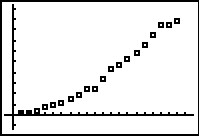
\includegraphics[width=2in]{./ExpLogsGraphics/Applications05.jpg}}

%Which models are suggested by the shape of the data?  Thinking back Section \ref{Regression}, we try a Quadratic Regression, with pretty good results.

%\begin{center}

%\begin{tabular}{cc}

%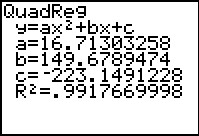
\includegraphics[width=2in]{./ExpLogsGraphics/Applications06.jpg} &

%\hspace{0.75in} 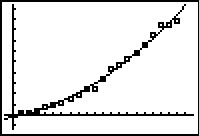
\includegraphics[width=2in]{./ExpLogsGraphics/Applications07.jpg} \\

%\end{tabular}

%\end{center}

%However, is there any scientific reason for the data to be quadratic?  Are there other models which fit the data equally well, or better?  Scientists often use logarithms in an attempt to `linearize' data sets - in other words, transform the data sets to produce ones which result in straight lines.  To see how this could work, suppose we guessed the relationship between $N$ and $t$ was some kind of power function, not necessarily quadratic, say $N = B t^{A}$.  To try to determine the $A$ and $B$, we can take the natural log of both sides and get $\ln(N) = \ln\left(B t^{A}\right)$.  Using properties of logs to expand the right hand side of this equation, we get $\ln(N) = A \ln(t) + \ln(B)$.  If we set $X = \ln(t)$ and $Y = \ln(N)$, this equation becomes $Y = AX + \ln(B)$.  In other words, we have a line with slope $A$ and $Y$-intercept $\ln(B)$.  So, instead of plotting $N$ versus $t$, we plot $\ln(N)$ versus $\ln(t)$.

%\[ \begin{array}{|c||c|c|c|c|c|c|c|c|c|c|c|c|c|}  \hline

%\ln(t) & 0 & 0.693 & 1.099 & 1.386& 1.609 & 1.792 & 1.946 & 2.079 & 2.197 & 2.302 & 2.398 & 2.485 & 2.565  \\ \hline

%\ln(N) & 4.997  & 5.549 &  5.905 & 6.489 & 6.800 & 6.989 & 7.306 & 7.546 & 7.771 & 7.824 & 8.143 & 8.385 & 8.454  \\ \hline \end{array} \]


%\[\begin{array}{|c||c||c|c|c|c|c|c|} \hline

%\ln(t) & 2.639 & 2.708 & 2.773 & 2.833 & 2.890 & 2.944 & 2.996  \\ \hline 

%\ln(N) & 8.566 & 8.653 & 8.779 & 8.925 & 9.042 & 9.045 & 9.086    \\ \hline \end{array} \]

%Running a linear regression on the data gives

%\begin{center}

%\begin{tabular}{cc}

%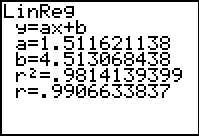
\includegraphics[width=2in]{./ExpLogsGraphics/Applications08.jpg} &

%\hspace{0.75in} 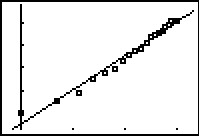
\includegraphics[width=2in]{./ExpLogsGraphics/Applications09.jpg} \\

%\end{tabular}

%\end{center}

%The slope of the regression line is $a \approx 1.512$ which corresponds to our exponent $A$.  The $y$-intercept $b \approx 4.513$ corresponds to $\ln(B)$, so that $B \approx 91.201$.  Hence, we get the model $N = 91.201 t^{1.512}$, something from Section \ref{AlgebraicFunctions}.  Of course, the calculator has a built-in `Power Regression' feature.  If we apply this to our original data set, we get the same model we arrived at before.\footnote{Critics may question why the authors of the book have chosen to even discuss linearization of data when the calculator has a Power Regression built-in and ready to go.  Our response:  talk to your science faculty.}


%\begin{center}

%\begin{tabular}{cc}

%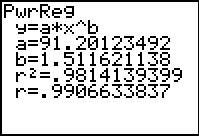
\includegraphics[width=2in]{./ExpLogsGraphics/Applications10.jpg} &

%\hspace{0.75in} 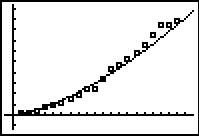
\includegraphics[width=2in]{./ExpLogsGraphics/Applications11.jpg} \\

%\end{tabular}

%\end{center}

%This is all well and good, but the quadratic model appears to fit the data better, and we've yet to mention any scientific principle which would lead us to believe the actual spread of the flu follows any kind of power function at all.  If we are to attack this data from a scientific perspective, it does seem to make sense that, at least in the early stages of the outbreak, the more people who have the flu, the faster it will spread, which leads us to proposing an uninhibited growth model. If we assume $N = B e^{At}$ then, taking logs as before, we get $\ln(N) = At + \ln(B)$.  If we set $X = t$ and $Y = \ln(N)$, then, once again, we get $Y = AX + \ln(B)$, a line with slope $A$ and $Y$-intercept $\ln(B)$.  Plotting $\ln(N)$ versus $t$ gives the following linear regression.  

%\phantomsection
%\label{swineflulinearized}

%\begin{center}

%\begin{tabular}{cc}

%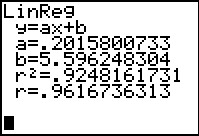
\includegraphics[width=2in]{./ExpLogsGraphics/Applications12.jpg} &

%\hspace{0.75in} 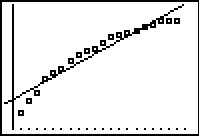
\includegraphics[width=2in]{./ExpLogsGraphics/Applications13.jpg} \\

%\end{tabular}

%\end{center}

%We see the slope is  $a \approx 0.202$ and which corresponds to $A$ in our model, and the $y$-intercept is $b \approx 5.596$ which corresponds to $\ln(B)$.  We get $B \approx 269.414$, so that our model is $N = 269.414e^{0.202t}$. Of course, the calculator has a built-in `Exponential Regression' feature which produces what appears to be a different model $N = 269.414 (1.22333419)^{t}$.  Using properties of exponents, we write $e^{0.202t} = \left(e^{0.202}\right)^t \approx (1.223848)^{t}$, which, had we carried more decimal places, would have matched the base of the calculator model exactly.

 
%\begin{center}

%\begin{tabular}{cc}

%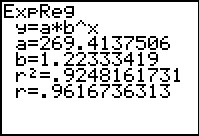
\includegraphics[width=2in]{./ExpLogsGraphics/Applications14.jpg} &

%\hspace{0.75in} 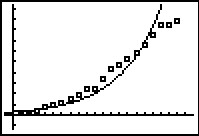
\includegraphics[width=2in]{./ExpLogsGraphics/Applications15.jpg} \\

%\end{tabular}

%\end{center}

%The exponential model didn't fit the data as well as the quadratic or power function model, but it stands to reason that, perhaps, the spread of the flu is not unlike that of the spread of a rumour and that a logistic model can be used to model the data.  The calculator does have a `Logistic Regression' feature, and using it produces the model $N = \frac{10739.147}{1 + 42.416 e^{0.268 t}}$.

%\begin{center}

%\begin{tabular}{cc}

%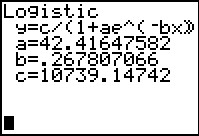
\includegraphics[width=2in]{./ExpLogsGraphics/Applications16.jpg} &

%\hspace{0.75in} 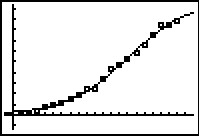
\includegraphics[width=2in]{./ExpLogsGraphics/Applications17.jpg} \\

%\end{tabular}

%\end{center}

%This appears to be an excellent fit, but there is no friendly coefficient of determination, $R^2$, by which to judge this numerically.  There are good reasons for this, but they are far beyond the scope of the text.  Which of the models, quadratic, power, exponential, or logistic is the `best model'?  If by `best' we mean `fits closest to the data,' then the quadratic and logistic models are arguably the winners with the power function model a close second.  However, if we think about the science behind the spread of the flu, the logistic model gets an edge.  For one thing, it takes into account that only a finite number of people will ever get the flu (according to our model, $10,\!739$), whereas the quadratic model predicts no limit to the number of cases. As we have stated several times before in the text, mathematical models, regardless of their sophistication, are just that:  models, and they all have their limitations.\footnote{Speaking of limitations, as of June 3, 2009, there were 19,273 confirmed cases of influenza A (H1N1).  This is well above our prediction of 10,739.  Each time a new report is issued, the data set increases and the model must be recalculated.  We leave this recalculation to the reader.}



\printexercises{exercises_pre/06_05_exercises}